\documentclass[11pt,a4paper]{article}
\usepackage{{../../paquete-formulas}}
\usepackage{{../../estilos-formulas}}
\usepackage[thinlines]{easytable} %Para tener comando TAB y tablas dif.


\newcommand{\materia}{Máquinas Térmicas}
\newcommand{\vs}{\vspace{-.3cm}}


\begin{document}
	\pagestyle{pieyencabezado}
	
	\section*{Nomenclatura}
	\begin{tabular}{r l}
		PCI [kcal/kg$_{comb}$] & Poder calorífico inferior \\
		PCS [kcal/kg$_{comb}$] & Poder calorífico superior \\
		H, S, C, O & \% del elemento en peso por kilogramo de combustible (cant. centesimal)\\
		H$_2$O & \% de humedad en el combustible \\
		G & Peso\\
		m & Masa\\
		C & Calor latente\\
		c$_p$ & Calor específico
	\end{tabular}

	\unidad{2}{Combustibles para generadores de calor}
	
	\begin{multicols}{2}
		\begin{cajita}
			
			\subtitulo{Poder calorífico}
			
			\vspace{.2cm}
			
			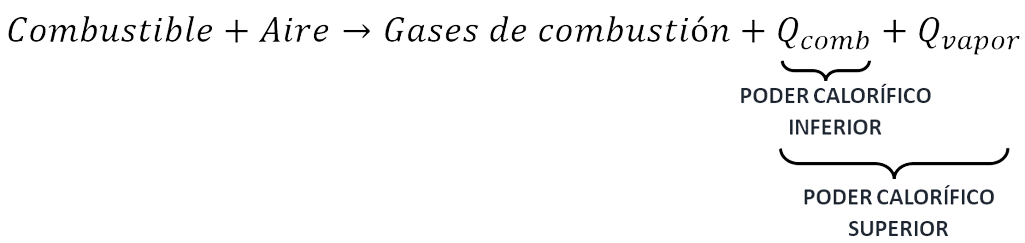
\includegraphics[width = \linewidth]{U2-poderes-calorificos}\vs
			
			\begin{flushleft}
				Relación entre los poderes caloríficos
			\end{flushleft}\vspace{-.2cm}
			
			$PCI = PCS - Q_{vapor} = PCS - 579 G$\vspace{.2cm}
			
			
			\boxed{PCI = PCS - 579 \left(9H+H_2O\right)}\vspace{.2cm}
			
			\begin{tabular}{r p{.7\linewidth}}
				$Q_{vapor}$ & Calor de condensación del vapor de agua\\
				$G$ & \% en peso del agua formada por la combustión más la humedad del combustible.\\
				$597$ & Calor de condensación del agua a $0^\circ C$.
			\end{tabular}
			
			\subsubtitulo{Hidrógeno}
			\vspace{-.8cm}
			
			
			\begin{flushleft}
				Reacción química de la combustión completa del hidrógeno
			\end{flushleft}\vs
			
			$H_2 + \frac{1}{2}O_2 \rightarrow H_2O + \boxed{34400} \left[\frac{kcal}{kg_H}\right]$
		
		\subsubtitulo{Carbono}
		\vspace{-.8cm}
		
		\begin{flushleft}
			Reacción química de la combustión completa del carbono
		\end{flushleft}\vs
	
		$C + O_2 \rightarrow CO_2 + \boxed{8140} \left[\frac{kcal}{kg_C}\right]$
		
		\begin{flushleft}
			Reacción química de la combustión incompleta del carbono
		\end{flushleft}\vs
	
		$C + \frac{1}{2} O_2 \rightarrow CO + \boxed{2440} \left[\frac{kcal}{kg_C}\right]$
			
		\subsubtitulo{Azufre}
		\vspace{-.8cm}
		
		\begin{flushleft}
			Reacción química de la combustión para el azufre.
		\end{flushleft}\vs
	
		$S + O_2 \rightarrow SO_2 + \boxed{2220} \left[\frac{kcal}{kg_S}\right] $
		
		\end{cajita}
		\columnbreak
		\begin{cajita}
			\subtitulo{Método analítico}
			
			\subsubtitulo{Fórmula de Dulong}
			\vspace{-.8cm}
			
			\begin{flushleft}
				PC de un combustible seco
			\end{flushleft}
			
			\vspace{-.2cm}
		
			\boxed{PCS = PCI = 8140  C + 34400 \left(H - \dfrac{O}{8} \right) + 2220 S}
			
			\begin{flushleft}
				PCI de un combustible húmedo
			\end{flushleft}
			
			\vspace{-.2cm}
			
			\boxed{PCI = 8140  C + 34400 \left(H - \dfrac{O}{8} \right) + 2220 S - 600 H_2O}
			
			\subsubtitulo{Fórmula de Hutte}
			
			\vspace{-.8cm}
			
			\begin{flushleft}
				PCS de un combustible húmedo
			\end{flushleft}
		
			\vspace{-.2cm}
			
			\boxed{PCI = 8100  C + 29000 \left(H - \dfrac{O}{8} \right) + 2500 S - 600 H_2O}
			
			\subsubtitulo{Fórmula de la Asociación de Ingenieros Alemanes}
			
			\vspace{-.8cm}
			
			\begin{flushleft}
				PCI de un combustible húmedo
			\end{flushleft}
			
			\vspace{-.2cm}
			
			\boxed{PCI = 8080  C + 29000 \left(H - \dfrac{O}{8} \right) + 2500 S - 600 H_2O}
			\vspace{.2cm}
			
			\begin{tabular}{r p{.7\linewidth}}
				$\dfrac{O}{8}$ & \% de $H_2$ en peso combinado con el $O_2$ del combustible dando \emph{agua de combinación}\\
				$H - \dfrac{O}{8}$ & \% de \emph{hidrógeno disponible} en peso que se oxida con el aire ($O_2$) para dar \emph{agua de formación}
			\end{tabular}
		\end{cajita}
	\end{multicols}
	
	\begin{cajita}
		
		\subtitulo{Método práctico}
		
		\subsubtitulo{Calorímetro de Mahler y Kroeker}\vspace{-.6cm}
		
		\begin{multicols}{2}
			\begin{flushleft}
				Supone que el calor $Q$ generado dentro de la bomba calorimétrica es absorbido por los elementos que la rodean:
				\begin{itemize}
					\item Agua contenida\\[.1cm]
					\item Agitador\\[.1cm]
					\item Termómetro\\[.1cm]
					\item Bomba\\[.1cm]
					\item Recipiente
				\end{itemize} 
			
				Y dicho calor es cedido por la combustión y el alambre:
			\end{flushleft} 
			\begin{tabular}{r c l}
				$Q$ & = & $Q_{combustible} + Q_{alambre}$\\[.2cm]
					& = & $\left(m_{w} {c_p}_{w} + E_{aparato}\right) \Delta t$\\[.2cm]
			\end{tabular}
			
			
			
			$PCS = \dfrac{Q_{comb}}{G_{comb}}$\\[.1cm]
			
				\columnbreak
			
			\boxed{PCS = \dfrac{\left(m_{w} {c_p}_{w} + E_{aparato}\right) \Delta t - m_{alam} C_{alam}}{G_{comb}}}\\[.1cm]
			\boxed{PCI = PCS - 600 \dfrac{G_w}{G_{comb}}}
			\vspace{.3cm}
		
			
			\begin{tabular}{r p{.7\linewidth}}
				$G_w$ & Peso total de agua existente $= papel\,húmedo - papel\, seco$\\
				$G_{comb}$ & Peso de combustible quemado\\
			\end{tabular}
		\end{multicols}
		
	\end{cajita}
	
	\begin{cajita}
			
		\begin{center}
			\subtitulo{Aire mínimo para una combustión perfecta}
		\end{center}
		\begin{equation}
			G_{t \ aire} = 11.6 g_{c} + 34.78 g_{hd} +4.35 g_{s} \; [Kg_{aire}/Kg_{comb.}]
		\end{equation}
		\begin{equation}
			V_{t \ aire} = 8.89 g_{c} + 26.27 g_{hd} + 3.34 g_{s} \; [m^{3}_{aire}/Kg_{comb.}]
		\end{equation}
		\begin{flushleft}
			Donde 
		
		$g_{hd} = g_{h} - \dfrac{g_{o_{2}}}{2}$
		
		$g_{c}$ composición gravimétrica carbono
		
		$g_{h}$ composición gravimétrica hidrógeno
		
		$g_{o_{2}}$ composición gravimétrica oxígeno
		
		$g_{s}$ composición gravimétrica azufre
		
		-
		\\
	
		En la práctica es necesario trabajar con un exceso de aire para que asegurar la combustión perfecta:
		\end{flushleft}
		\begin{equation}
			V_{R \ aire} = (1+e) V_{t \ aire} [m^{3}_{aire}/Kg_{comb.}]
		\end{equation}
		
		
		\end{cajita}
		\begin{cajita}
		
		\begin{center}
			\subtitulo{Gases de combustión}
		\end{center}
		\begin{equation}
			g_{h} = (3.67 g_{c} + 9 g_{hd} +2 g_{s}) + 3.35 (2.67 g_{c} + 8 g_{hd} + g_{s}) + g_{w} \; [Kg_{humo}/Kg_{comb}]
		\end{equation}
		\begin{equation}
			V_{h} = 1.897 g_{c} + 11.2 g_{hd} +0.7 g_{s} + 3.76 (1.867 g_{c} + 5.6 g_{hd} +0.7 g_{s}) + 1.24 g_{w} \; [m^{2}_{humo}/Kg_{comb}]
		\end{equation}
	\end{cajita}
	
	\begin{cajita}
		\subtitulo{Exceso de aire}
		\begin{multicols}{2}
			\begin{tabular}{r p{0.87\textwidth}}
				$g_{h}$ & (kg de gases húmedos/ kg de combustible)\\
				$e$ & (coeficiente de exceso de aire)\\
				$g'_{S}$ & (kg gases secos / kg carbono)\\
				$g''_{S}$ & (kg gases secos / kmol combustible)\\
				$\mu$ & (masa molecular) (kg/kmol)\\
				$G_{AT}$ & (kg de aire teórico / kg de combustible)\\
				$g_{S}$ & (kg gases secos/ kg de combustible)\\
				$g_{C}$ & kg de carbono / kg de combustible)\\
				$g'_{C}$ & (kg carbono / kmol combustible)\\
				$g{w}$ & (kg de aire teórico/ kg combustible)\\
				$r$ & composición volumentrica\\
				
			\end{tabular}
			\begin{tabular}{r l }
			$g_{h}=$&$1+e~G_{AT}$\\[0.2cm]
			$e=$&$\dfrac{g_{h}-1}{G_{AT}}$\\
			$g_{h}=$&$g_{s}+g_{w}$\\
			$g_{S}=$&$g'_{S}~g_{C}$\\
			\end{tabular}
			\begin{tabular}{r l }
				$g'_{S}=$&$\dfrac{G''_{S}}{g'_{C}}$\\
				$g_{i}=$&$\mu_{i}~r_{i}$\\[0.3cm]
				$g''_{S}=$&$\displaystyle \sum_{i=1}^{n} \mu_{i}~r_{i}$\\[0.3cm]
				$g'_{C}=$&$\displaystyle \sum_{i=1}^{n} \mu_{C}~r_{iC}$\\[0.3cm]
				$g'_{S}=$&$\dfrac{\sum_{i=1}^{n} \mu_{i}~r_{i}}{\sum_{i=1}^{n} \mu_{C}~r_{iC}}$\\[0.3cm]
				$g_{h}=$&$\dfrac{\sum_{i=1}^{n} \mu_{i}~r_{i}}{\sum_{i=1}^{n} \mu_{C}~r_{iC}} g_{C}+g_{w}$\\[0.35cm]
				$g_{w}=$&$9~g_{he}$\\[0.1cm]
				$G_{AT}=$&$11.6~g_{C}+37.38~g_{hd}+4.35~g_{S}$\\
				&\tiny{para mi aca gs es del azufre, no gases secos/comb.}
			\end{tabular}
		\end{multicols}
	Yo copié las formulas, pero los analisis dimensionales no dan en algunos...
	\end{cajita}
		
	% \newpage
	\begin{cajita}
		\subtitulo{ Caracteristica de una caldera}
		\renewcommand{\arraystretch}{1.25}
		\begin{multicols}{2}
			% \begin{tabular}{l{1cm} l{5cm}}
			% asdasdads& asdasdasd\\			
			% \end{tabular}
			\begin{tabular}{@{}p{1cm}@{}@{}p{7cm}@{}}
				$G_{r}$ & cantidad vapor producido\\
	
				$R_{e}$&relacion estequio... 9,7 para gas natural\\
				$\lambda$&exceso de aire $\dfrac{21}{21-O_{2}}$\\
				$v$ & velocidad gas\\
				$A_{2}$y$B$& parametros dependen gas/caldera?\\
				$P_{ab}$ & va en MCA\\
				$P_C$& en combustible sin quemar es la potencia calorifica del carbono, 8140 $kcal/kg$\\
				$\% C$ & es Carbono sin quemar, en las cenizas\\
			\end{tabular}
	
			\renewcommand{\arraystretch}{1.5}
	
			PERDIDAS\\
	
			\begin{tabular}{r l}
				gases comb & $Q = G_{g} c_{p~\textit{humo}} (t_{gas}-t_{aire})$\\
				humedad comb & $ Q= G_{h2o} \Delta h_{agua}$\\
				comb sin quemar & $ Q =\dfrac{G_{escoria}}{G_{combustible}}~P_{C}~\% C$\\
				hw comb comb &$ Q=9~G_{humedad} ~\Delta h_{agua}$\\
				exceso aire & $Q = G_{aire}~c_{p~\textit{humo}} (t_{gas}-t_{aire})$\\
			\end{tabular}
			
			\renewcommand{\arraystretch}{1.5}
		
			\begin{tabular}{r l}
				Capacidad  & $Q=G_{r} \, \Delta h$\\
				Potencia  (HP) & $P=\dfrac{G_{v}\,\left(\Delta h\right)}{543.4(kcal/kg)~~15.66(kg)}~~$\\
				&$~~=\dfrac{G_{v}\,\left(\Delta h\right)}{8510 (kcal/hp~h)}$\\[0.4cm]
				Aire combustion& $A_{c}=G_{c}\,Re\,\lambda$\\
				% \multicolumn{2}{r}{\begin{itemize}
				% 	\item ASD
				% \end{itemize}}\\
				\multicolumn{2}{c}{\textsl{Ejercicio dimensionamieto?}}\\
				Diametro tubo gas & $D=\sqrt{\dfrac{365.35\,G_{c}}{v~~P_{ab}}}~~$ \textit{(v<40m/s)}\\
				Presión abs gas& $P_{ab}=P_{atm}+P_{carga}+P_{contra}$\\
				Perdida gases & $pg=(T_{gas}-T_{amb})\left(\dfrac{A_{2}}{21-O_{2}}+B\right)$\\
				Rendimiento  & $ \eta=100-pg$\\
				Calor quemador& $Q=\dfrac{G_{v}(\Delta H)}{\eta_{caldera} \, n_{quemadores}}$\\
			\end{tabular}
		\end{multicols}
	
			\begin{center}
				\textbf{Intercambiador (superficies de intercambio)}
			\end{center}
	
			\begin{multicols}{2}
				\renewcommand{\arraystretch}{1}
				\begin{tabular}{@{}p{1cm}@{}@{}p{7cm}@{}}
					$S$ & superficie de intercambio\\
					$n$ & número de tubos\\
					$l$ & longitud tubos\\
					$d$& diametro tubos\\
					$K$ & coef total de transmisión de calor\\
					$\alpha$ & coeficientes peliculares \break (humo/vapor/agua)\\
				\end{tabular}
				
				\renewcommand{\arraystretch}{1.5}
				\begin{tabular}{l l}
					$S=n~l~\pi~d$ &	$Q=S~K~\Delta T_m$\\[0.2cm]
					$\Delta T_m = \dfrac {\Delta T_1 - \Delta T_2}{ln\left(\frac{\Delta T_1}{\Delta T_2}\right)}$ & $K=\dfrac{1}{\dfrac{1}{\alpha_1}+\dfrac{e}{\lambda}+\dfrac{1}{\alpha_2}}$\\
				\end{tabular}\\
				\renewcommand{\arraystretch}{1}
				\begin{tabular}{@{}p{1cm}@{}@{}p{7cm}@{}}
					$e$& espesor tubo\\
					$\Delta T_m$ & diferencia log de temp\\
					$\lambda$ & conductividad térmica tubo\\
	
				\end{tabular}
			\end{multicols}
		\end{cajita}

\end{document}\begin{cajita}
	\subtitulo{ Caracteristica de una caldera}
	\renewcommand{\arraystretch}{1.25}
	\begin{multicols}{2}
		% \begin{tabular}{l{1cm} l{5cm}}
		% asdasdads& asdasdasd\\			
		% \end{tabular}
		\begin{tabular}{@{}p{1cm}@{}@{}p{7cm}@{}}
			$G_{r}$ & cantidad vapor producido\\

			$R_{e}$&relacion estequio... 9,7 para gas natural\\
			$\lambda$&exceso de aire $\dfrac{21}{21-O_{2}}$\\
			$v$ & velocidad gas\\
			$A_{2}$y$B$& parametros dependen gas/caldera?\\
			$P_{ab}$ & va en MCA\\
			$P_C$& en combustible sin quemar es la potencia calorifica del carbono, 8140 $kcal/kg$\\
			$\% C$ & es Carbono sin quemar, en las cenizas\\
		\end{tabular}

		\renewcommand{\arraystretch}{1.5}

		PERDIDAS\\

		\begin{tabular}{r l}
			gases comb & $Q = G_{g} c_{p~\textit{humo}} (t_{gas}-t_{aire})$\\
			humedad comb & $ Q= G_{h2o} \Delta h_{agua}$\\
			comb sin quemar & $ Q =\dfrac{G_{escoria}}{G_{combustible}}~P_{C}~\% C$\\
			hw comb comb &$ Q=9~G_{humedad} ~\Delta h_{agua}$\\
			exceso aire & $Q = G_{aire}~c_{p~\textit{humo}} (t_{gas}-t_{aire})$\\
		\end{tabular}
		
		\renewcommand{\arraystretch}{1.5}
	
		\begin{tabular}{r l}
			Capacidad  & $Q=G_{r} \, \Delta h$\\
			Potencia  (HP) & $P=\dfrac{G_{v}\,\left(\Delta h\right)}{543.4(kcal/kg)~~15.66(kg)}~~$\\
			&$~~=\dfrac{G_{v}\,\left(\Delta h\right)}{8510 (kcal/hp~h)}$\\[0.4cm]
			Aire combustion& $A_{c}=G_{c}\,Re\,\lambda$\\
			% \multicolumn{2}{r}{\begin{itemize}
			% 	\item ASD
			% \end{itemize}}\\
			\multicolumn{2}{c}{\textsl{Ejercicio dimensionamieto?}}\\
			Diametro tubo gas & $D=\sqrt{\dfrac{365.35\,G_{c}}{v~~P_{ab}}}~~$ \textit{(v<40m/s)}\\
			Presión abs gas& $P_{ab}=P_{atm}+P_{carga}+P_{contra}$\\
			Perdida gases & $pg=(T_{gas}-T_{amb})\left(\dfrac{A_{2}}{21-O_{2}}+B\right)$\\
			Rendimiento  & $ \eta=100-pg$\\
			Calor quemador& $Q=\dfrac{G_{v}(\Delta H)}{\eta_{caldera} \, n_{quemadores}}$\\
		\end{tabular}
	\end{multicols}

		\begin{center}
			\textbf{Intercambiador (superficies de intercambio)}
		\end{center}

		\begin{multicols}{2}
			\renewcommand{\arraystretch}{1}
			\begin{tabular}{@{}p{1cm}@{}@{}p{7cm}@{}}
				$S$ & superficie de intercambio\\
				$n$ & número de tubos\\
				$l$ & longitud tubos\\
				$d$& diametro tubos\\
				$K$ & coef total de transmisión de calor\\
				$\alpha$ & coeficientes peliculares \break (humo/vapor/agua)\\
			\end{tabular}
			
			\renewcommand{\arraystretch}{1.5}
			\begin{tabular}{l l}
				$S=n~l~\pi~d$ &	$Q=S~K~\Delta T_m$\\[0.2cm]
				$\Delta T_m = \dfrac {\Delta T_1 - \Delta T_2}{ln\left(\frac{\Delta T_1}{\Delta T_2}\right)}$ & $K=\dfrac{1}{\dfrac{1}{\alpha_1}+\dfrac{e}{\lambda}+\dfrac{1}{\alpha_2}}$\\
			\end{tabular}\\
			\renewcommand{\arraystretch}{1}
			\begin{tabular}{@{}p{1cm}@{}@{}p{7cm}@{}}
				$e$& espesor tubo\\
				$\Delta T_m$ & diferencia log de temp\\
				$\lambda$ & conductividad térmica tubo\\

			\end{tabular}
		\end{multicols}